\documentclass[tikz,border=4pt]{standalone}
% Shared style for every figure and for the deck: one accent, one
% highlight, thin lines, rounded nodes, nothing decorative.
\usepackage[T1]{fontenc}
\usepackage{lmodern}
\renewcommand{\familydefault}{\sfdefault}
\usepackage{tikz}
\usetikzlibrary{arrows.meta,positioning,calc,shapes.misc,fit,backgrounds,decorations.pathreplacing}
\definecolor{ink}{RGB}{40,40,40}
\definecolor{soft}{RGB}{150,150,150}
\definecolor{faint}{RGB}{225,225,225}
\definecolor{accent}{RGB}{0,95,115}
\definecolor{accentlight}{RGB}{214,232,236}
\definecolor{warn}{RGB}{196,84,40}
\definecolor{warnlight}{RGB}{247,226,216}
\tikzset{
  every picture/.style={color=ink, line width=0.5pt, font=\small},
  node distance=12mm and 18mm,
  box/.style={draw=ink, rounded corners=2pt, fill=white, inner sep=5pt, minimum height=7mm, align=center},
  maker/.style={box, minimum width=18mm},
  cat/.style={box, inner sep=3.5pt, minimum height=6mm},
  root/.style={box, fill=accentlight, draw=accent},
  bad/.style={box, fill=warnlight, draw=warn},
  ghost/.style={box, draw=soft, text=soft, dashed},
  flow/.style={-{Stealth[length=4pt,width=3.5pt]}, line width=0.5pt},
  sub/.style={-{Stealth[length=4pt,width=3.5pt]}, line width=0.5pt, color=soft},
  strong/.style={flow, color=accent, line width=0.8pt},
  wrong/.style={flow, color=warn},
  lbl/.style={font=\footnotesize, text=ink, inner sep=1.5pt, fill=white},
  note/.style={font=\footnotesize, text=soft, align=center},
  rate/.style={font=\footnotesize, text=accent, inner sep=1pt, fill=white},
}

\usepackage{amsmath}
\usepackage{pgfplots}
\pgfplotsset{compat=1.17}

\begin{document}
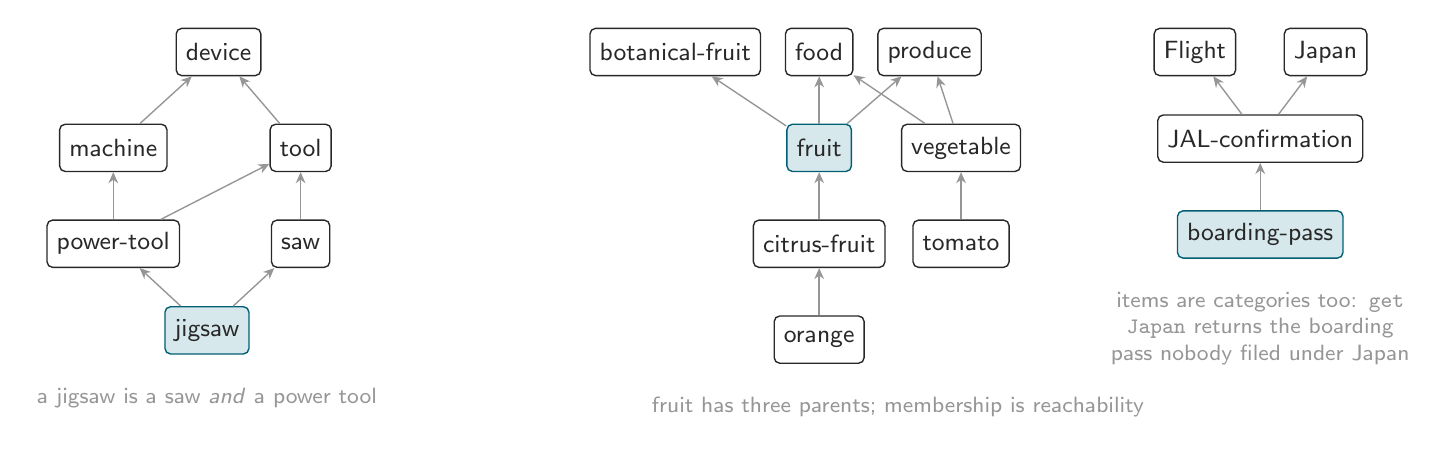
\begin{tikzpicture}[node distance=6mm and 4mm]
  % Three small DAGs from ontodag's core pack (real edges). Supercategories
  % above, subcategories below; every arrow points up.
  \begin{scope}
    \node[cat] (device) {device};
    \node[cat, below left=6mm and 1mm of device] (machine) {machine};
    \node[cat, below right=6mm and 1mm of device] (tool) {tool};
    \node[cat, below=6mm of machine] (power) {power-tool};
    \node[cat, below=6mm of tool] (saw) {saw};
    \node[cat, fill=accentlight, draw=accent] (jigsaw) at ($(power)!0.5!(saw) + (0,-11mm)$) {jigsaw};
    \draw[sub] (machine) -- (device); \draw[sub] (tool) -- (device);
    \draw[sub] (power) -- (machine); \draw[sub] (power) -- (tool);
    \draw[sub] (saw) -- (tool);
    \draw[sub] (jigsaw) -- (power); \draw[sub] (jigsaw) -- (saw);
    \node[note, below=3mm of jigsaw] {a jigsaw is a saw \emph{and} a power tool};
  \end{scope}
  \begin{scope}[xshift=58mm]
    \node[cat] (bot) {botanical-fruit};
    \node[cat, right=3mm of bot] (food) {food};
    \node[cat, right=3mm of food] (produce) {produce};
    \node[cat, below=6mm of food, fill=accentlight, draw=accent] (fruit) {fruit};
    \node[cat, below=6mm of produce, xshift=4mm] (veg) {vegetable};
    \node[cat, below=6mm of fruit] (citrus) {citrus-fruit};
    \node[cat, below=6mm of veg] (tomato) {tomato};
    \node[cat, below=6mm of citrus] (orange) {orange};
    \draw[sub] (fruit) -- (bot); \draw[sub] (fruit) -- (food); \draw[sub] (fruit) -- (produce);
    \draw[sub] (veg) -- (food); \draw[sub] (veg) -- (produce);
    \draw[sub] (citrus) -- (fruit); \draw[sub] (orange) -- (citrus); \draw[sub] (tomato) -- (veg);
    \node[note, below=3mm of orange, xshift=10mm] {fruit has three parents; membership is reachability};
  \end{scope}
  \begin{scope}[xshift=124mm]
    \node[cat] (flight) {Flight};
    \node[cat, right=6mm of flight] (japan) {Japan};
    \node[cat] (jal) at ($(flight)!0.5!(japan) + (0,-11mm)$) {JAL-confirmation};
    \node[cat, below=6mm of jal, fill=accentlight, draw=accent] (pass) {boarding-pass};
    \draw[sub] (jal) -- (flight); \draw[sub] (jal) -- (japan); \draw[sub] (pass) -- (jal);
    \node[note, below=3mm of pass, text width=40mm] {items are categories too: \texttt{get Japan} returns the boarding pass nobody filed under Japan};
  \end{scope}
\end{tikzpicture}
\end{document}
